\documentclass{extarticle}
\usepackage[a4paper, margin=2cm]{geometry}
\usepackage{graphicx}
\graphicspath{{images/}}
\usepackage{float}
\usepackage{parskip}
\usepackage{xcolor}
\usepackage{listings}
\usepackage[os=mac]{menukeys}
\usepackage[colorlinks=true, linkcolor=cyan, citecolor=cyan, urlcolor=blue]{hyperref}
\lstset{
    basicstyle=\ttfamily,
    backgroundcolor=\color{gray!10},
    frame=single,
    rulecolor=\color{gray!50},
    columns=fullflexible
}

\setlength{\parskip}{1ex}

\title{OCaml Environment Setup}
\author{CSE 305 Introduction to Programming Languages}
\date{Fall 2025}

\begin{document}

\maketitle
\begin{center}
\textbf{Last Update:} \today
\end{center}

\section{Introduction}\label{Intro}
This document has a lot of information in it, we recommend you read through it before actually doing anything.
The order of operations is very important for setting up your environment, and the order of sections in this document is intentional.

We will cover installation instructions for different platforms in different sections.
Linux and macOS users should read Section~\ref{MacLinuxInstall},
and Windows users should read Section~\ref{DockerSetup}.


\newpage
\section{Installing OCaml on Linux/macOS}\label{MacLinuxInstall}

\subsection{macOS: Install package manager Homebrew}
Homebrew is the most popular `unofficial' package manager for macOS\@.
If you don't have it installed already, you should click on the \href{https://brew.sh/}{Homebrew website},
copy the install script and run it in \texttt{Terminal.app} or any terminal emulator you have.

\subsection{Install \texttt{opam}}
For macOS / Linux users, open any terminal emulator you have,
and use your package manager to install \texttt{opam}.

macOS:
\begin{lstlisting}
$ brew install opam
\end{lstlisting}

Debian/Ubuntu:
\begin{lstlisting}
$ sudo apt update & sudo apt upgrade -y
$ sudo apt install -y opam
\end{lstlisting}

When the installation is complete, run the following command in your terminal:
\begin{lstlisting}
$ opam init -a
\end{lstlisting}

When the installation is complete, restart your machine and open a new terminal.
Verify that the installation was successful by running \texttt{which ocaml} in your terminal,
it should look like this:
\begin{lstlisting}
$ which ocaml
<your_home_dir>/.opam/default/bin/ocaml
\end{lstlisting}

If the terminal says \texttt{ocaml: command not found},
it means there's something wrong with the initialization of \texttt{opam}.
Try to redo the steps and come to the office hours if the problem persists.

If the terminal says \texttt{/usr/bin/ocaml} or anything else not related to \texttt{.opam},
it means the system OCaml installation is being used instead of the one installed by \texttt{opam}.
You may need to restart your machine to make sure the system is reading the updated \texttt{.profile}.

If \texttt{which ocaml} prompt the path successfully, in your terminal run:
\begin{lstlisting}
$ opam switch create cse305_4.14.2 ocaml-base-compiler.4.14.2 && opam switch cse305_4.14.2
$ opam install -y ocaml-lsp-server ocamlformat utop
\end{lstlisting}

\subsection{Setting up text editor}
You can use whatever editor you are comfortable with.
However, we found VS Code to be the easiest editor to set up for use with OCaml.
\href{https://marketplace.visualstudio.com/items?itemName=ocamllabs.ocaml-platform}{OCaml Platform} is an extension we recommend for syntax highlighting and code auto completion.
The extension can be found in the VS Code Extension Store.

For macOS/Linux users, choose `cse305\_4.14.2' when VS Code asks for sandbox configuration.
This should enable syntax highlighting and autocomplete. Proceed to section~\ref{TestEnv} to test
your environment.


\newpage
\section{Using provided Docker images on Windows}\label{DockerSetup}
Setup for Windows is a little more complicated than other platforms,
so we provide a Docker image with all necessary tools,
Emacs development environment is also pre-installed.
We recommend using Visual Studio Code (VS Code) or Emacs as the text editor for this course.

\subsection{Install Docker Desktop}
Docker will prompt you several times to log in to an account, you \textbf{do not need a docker account} to use Docker
Desktop, or any of its features for this course.

Note that the Docker engine, and Docker Desktop \textbf{are not the same}, and we are supporting Docker Desktop.
You should go through \href{https://docs.docker.com/desktop/setup/install/windows-install/}{the documentation},
read through it first, and then follow the instructions to install Docker Desktop. You should also read through
\href{https://docs.docker.com/desktop/setup/install/windows-permission-requirements/}{this documentation}
if you have concerns about permissions on Windows.
In general, if you are unsure about a command you are running, you can find documentation using the man
pages, i.e. \texttt{man docker-build} or \texttt{man docker-run}, etc.

\subsection{Build the container from \texttt{cse305\_dev\_env} repository}
First, you need to clone the \href{https://github.com/UB-CSE-305/cse305_dev_env}{course repository}.
A Docker image is the standard for which Docker containers are built from. You should only have to build
this image once, and use it to create containers to develop within.

\subsubsection{Using Emacs in terminal}
You need to build and run the Docker image from the terminal.

While being in the same directory as the repository, you can build the image with the following command in a
terminal:
\begin{lstlisting}
$ docker build . -t 305image
\end{lstlisting}
You may replace \texttt{305image} with any appropriate name for how you want to organize it.
The \texttt{-t} flag in this instance refers to tagging the image with the name you provided.

To create a container from the image you just built:
\begin{lstlisting}
$ docker run --name 305container -it \
  --mount type=bind,source="$(pwd)"/local_workspace,target=/home/cse305/workspace \
  --user $(id -u):$(id -g) 305image
\end{lstlisting}
In this command, we are naming the container \texttt{305container}. The flags \texttt{-it} tell docker to run the container
with an interactive terminal.

\texttt{--mount} allows you to mount our \texttt{local\_workspace} folder into the container
at \texttt{/home/cse305/workspace}, and \texttt{--user \$(id -u):\$(id -g)} sets the user and group ID using
the current user's IDs to avoid permission issues. This setup allows most of the compilation and development work to happen within the Docker container,
while any code saved in the workspace folder inside the container actually resides on the host machine.
As a result, the code persists independently of the container lifecycle and will not be lost when the container is removed.
Therefore, the workspace folder \texttt{/home/cse305/workspace} is the primary location for you to develop your code.

\texttt{305image} being appended after the flags tells docker which image we want to create the container from.
After running that, you should shortly see something resembling a Linux command prompt.


If you have created a container before (and have not deleted it), you can run it with the following command:
\begin{lstlisting}
$ docker start -i 305container
\end{lstlisting}

To attach your current terminal session to the container:
\begin{lstlisting}
$ docker attach 305container
\end{lstlisting}

To list all containers you have created:
\begin{lstlisting}
$ docker ps -a
\end{lstlisting}
\texttt{-a} flag here shows all containers, including those that are stopped.

Pre-installed Emacs development environment provides out-of-the-box
Language Server Protocol (LSP) support and auto code formatting.
The red highlighting means that there's a syntax error, and LSP will provide
error/warning messages when you move your cursor to the highlighted code.
When you save the file (\texttt{C-x C-s}), \texttt{ocamlformat} will
automatically format your code if there are no syntax errors.

Some other useful Emacs commands when writing OCaml in the container:
\begin{itemize}
  \item \texttt{C-x C-l}: Jump to the definition of the symbol under cursor.
  \item \texttt{C-c C-i}: Jump to the declaration of the symbol under cursor.
  \item \texttt{C-c C-x}: Jump to next error in buffer.
  \item \texttt{C-c C-c}: Jump to previous error in buffer.
\end{itemize}

To add your own Emacs configurations, you should edit the file \textbf{\texttt{/home/cse305/.config/emacs/user.el}}.

Proceed to section~\ref{TestEnv} after setting up your preferred method.

\subsubsection{Using VS Code with plugins}
You need to install
\href{https://marketplace.visualstudio.com/items?itemName=ms-vscode-remote.remote-containers}{Dev Containers}
in order to access the full functionality if you are using Visual Studio Code.

We use the Dev Container plugin to connect the \texttt{/home/cse305/workspace} folder inside the Docker container with the \texttt{local\_workspace} in our repository.
This setup allows most of the compilation and development work to happen within the Docker container,
while any code saved in the workspace folder inside the container actually resides on the host machine.
As a result, the code persists independently of the container lifecycle and will not be lost when the container is removed.
Therefore, the workspace folder \texttt{/home/cse305/workspace} is the primary location for you to develop your code.

After installing the plugin, open the repository folder you just cloned in VS Code\@.
Then, open the VS Code Command Palette (\keys{\ctrl + p} or \keys{\cmd + p}) and
type \texttt{> Dev Container: Reopen in Container} to connect to your container.

\begin{figure}[H]
  \centering
  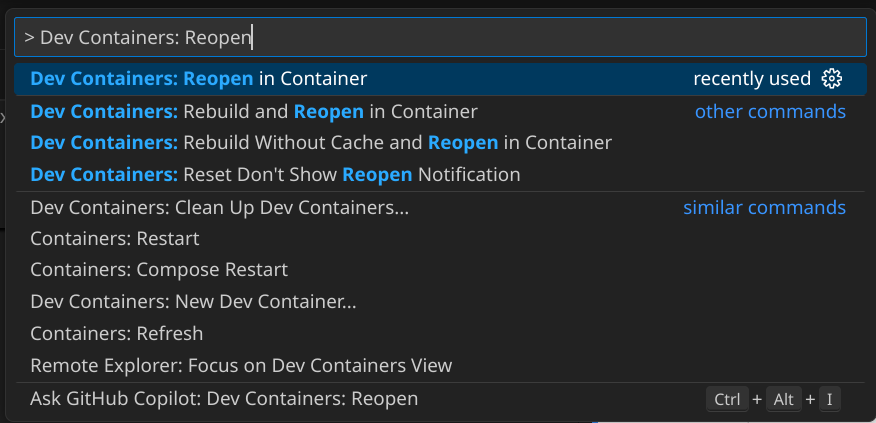
\includegraphics[width=0.6\textwidth]{vscode_cmd_pat.png}
\end{figure}

A new window will open and attach to the container. It will then pull and build the latest release image that matches your architecture and install the necessary extensions automatically.
Depending on your internet connection and system performance, this process may take some time.

\newpage
\section{Run your code}\label{CompileRun}
To run your OCaml code in the terminal, go to the correct directory with your \texttt{<filename.ml>} code file, and type:
\begin{lstlisting}
$ ocamlc -o <output_filename> <filename.ml>
$ ./<output_filename>
\end{lstlisting}

You can also run your OCaml code without compiling it first using the OCaml interpreter:
\begin{lstlisting}
$ ocaml <filename.ml>
\end{lstlisting}

Another way is to use the OCaml top-level \texttt{utop}, which is an interactive REPL environment.
After starting \texttt{utop}, you can run your code:
\begin{lstlisting}
#use "filename.ml";;
\end{lstlisting}
To exit \texttt{utop}:
\begin{lstlisting}
#quit;;
\end{lstlisting}
\begin{figure}[H]
  \centering
  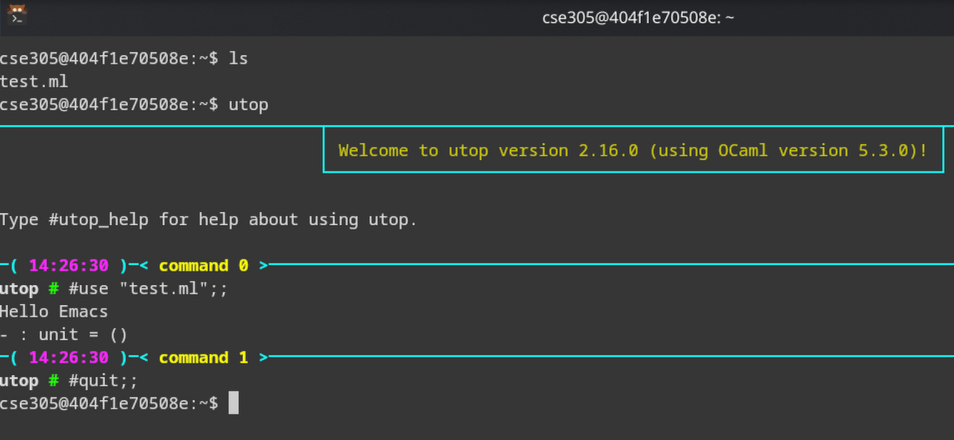
\includegraphics[width=0.6\textwidth]{utop_run_code.png}
\end{figure}
Check out section~\ref{TestEnv} for a concrete example.


\newpage
\section{Testing your environment}\label{TestEnv}
Open your text editor and create a file named \texttt{test.ml}. In the file write:
\begin{lstlisting}
print_endline "Hello, World!";;
\end{lstlisting}

Save your code, and then in your terminal navigate to the directory where you saved \texttt{test.ml}, and run:
\begin{lstlisting}
$ ocamlc -o hello test.ml
$ ./hello
\end{lstlisting}
This should print `Hello, World!' in the terminal:
\begin{figure}[H]
  \centering
  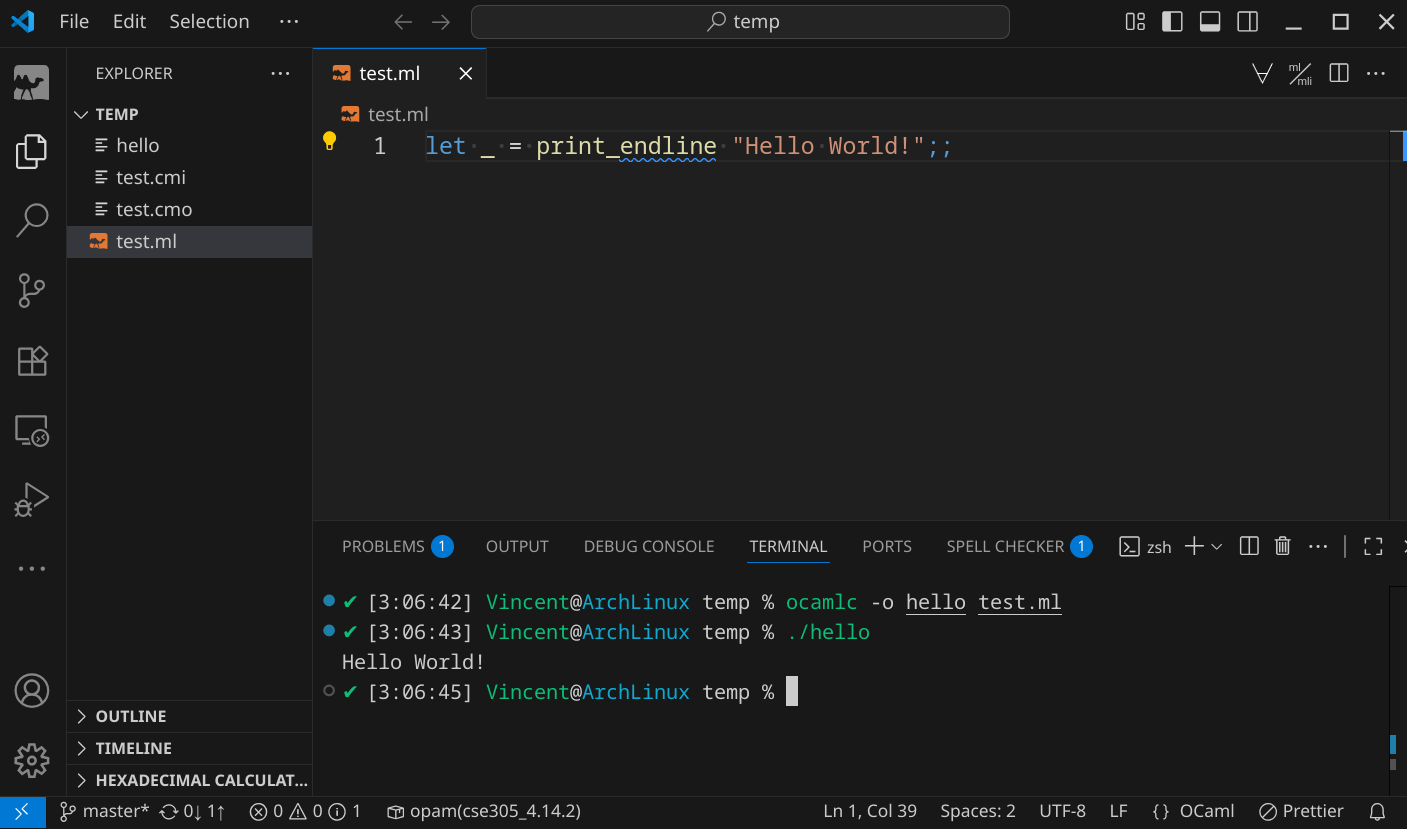
\includegraphics[width=0.6\textwidth]{compile_success.png}
\end{figure}

If your syntax highlighting and autocomplete are setup properly it should look like this:
\begin{figure}[H]
  \centering
  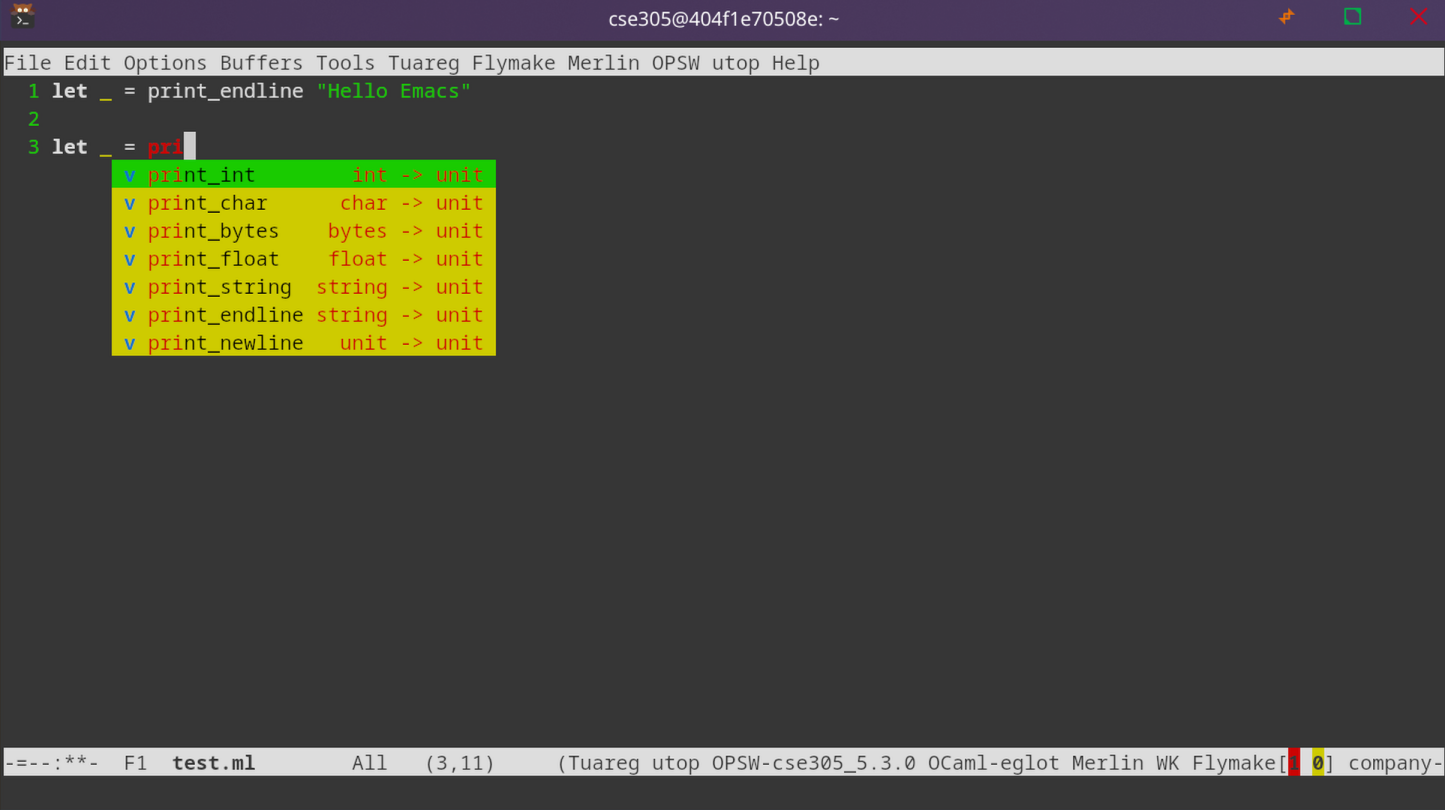
\includegraphics[width=0.6\textwidth]{emacs_autocomplete.png}
\end{figure}

When you write code with errors, \texttt{ocamllsp} will show static type errors in your text editor:
\begin{figure}[H]
  \centering
  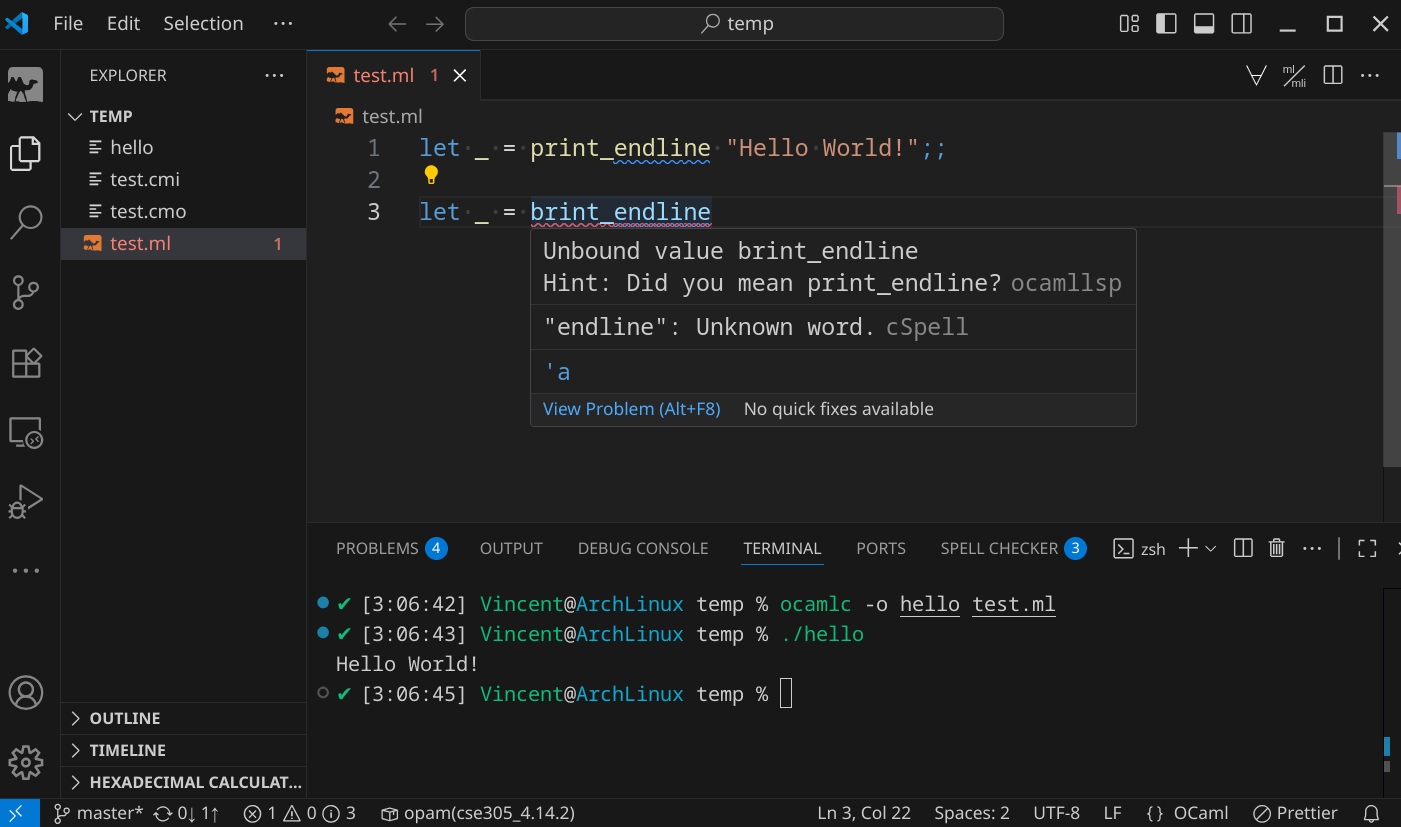
\includegraphics[width=0.6\textwidth]{static_check.png}
\end{figure}


\newpage
\section{Troubleshoot}\label{Troubleshoot}
\textbf{Q}: I ran \texttt{which ocaml} and it said \texttt{ocaml: command not found!}

\textbf{A}: If closing and reopening the terminal or restarting machine doesn't help,
run \texttt{opam env} in your terminal, normally it should look like this:
\begin{lstlisting}
[22:23:20] Vincent@ArchLinux ~ % opam env 
OPAM_LAST_ENV='/home/Vincent/.opam/.last-env/env-bf2bef-0'; export OPAM_LAST_ENV; 
OPAM_SWITCH_PREFIX='/home/Vincent/.opam/default'; export OPAM_SWITCH_PREFIX; 
CAML_LD_LIBRARY_PATH='/home/Vincent/.opam/default/lib/stublibs:
                      /home/Vincent/.opam/default/lib/ocaml/stublibs:
                      /home/Vincent/.opam/default/lib/ocaml'; export CAML_LD_LIBRARY_PATH; 
OCAML_TOPLEVEL_PATH='/home/Vincent/.opam/default/lib/toplevel'; export OCAML_TOPLEVEL_PATH; 
MANPATH=':/home/Vincent/.opam/default/man'; export MANPATH;
PATH='/home/Vincent/.opam/default/bin:/usr/local/sbin:/usr/local/bin:/usr/bin'; export PATH;
\end{lstlisting}
If the output is empty, something went wrong when \texttt{opam} initialized the environment.

If the output looks correct, but \texttt{which ocaml} still doesn't work,
You can manually add the following line to your shell configuration file
(\texttt{.bashrc}, \texttt{.zshrc}, etc.\ depending on which shell you are using,
you can find it out by running \texttt{echo \$SHELL}):
\begin{lstlisting}
eval $(opam env)
\end{lstlisting}
After adding that line, close and reopen your terminal and try \texttt{which ocaml} again.

\textbf{Q}: VSCode syntax highlighting and autocomplete not working

\textbf{A}: You need to install \texttt{ocaml-lsp-server} and \texttt{ocamlformat} by running:
\begin{lstlisting}
opam install -y ocaml-lsp-server ocamlformat
\end{lstlisting}

\textbf{Q}: I tried to build the Docker image, but it failed with an error.

\textbf{A}: Make sure you read the error message carefully.
It often provides clues about what went wrong.
Please let us know if you are unable to resolve the issue.

\newpage
\section{About}
The docker setup part of this document is adapted from CSE 421/521: Operating Systems,
and part of the Emacs setup configuration is adapted from \href{https://github.com/ub-cse220/emacs-config}{CSE 220: System Programming}.

\end{document}
